
\chapter{Bestärkendes Lernen }
Das bestärkende Lernen, auch Reinforcement Learning genannt ist neben dem überwachten Lernen und dem unüberwachten Lernen eine der Möglichkeiten des maschinellen Lernens . Es versucht aus den gegebenen Daten ohne anderes  vorhergehendes Wissen, Informationen zu gewinnen\cite[vgl.][S.7]{li2017deep}.
\label{NN}
\section{Funktionsweise}
\begin{center}
 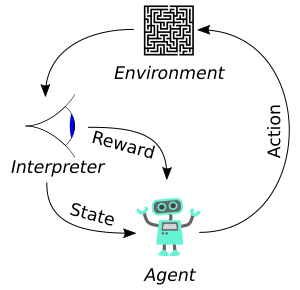
\includegraphics[scale = 1]{Bilder/Reinforcement_learning_diagram}\\
 \small{\textit{The typical framing of a Reinforcement Learning scenario}}\cite{RLdia}
\end{center}
Auf der Darstellung kann man die typische Funktionsweise des Bestärkenden Lernens erkennen.  Der Agent, nimmt eine Aktion, welche seine Umwelt beeinflusst. Daraufhin bekommt dieser wiederum die Information über den neuen Zustand (state) der Umwelt (enviroment) und eine Belohnung (reward), die auch negativ sein kann. Diese Schleife kann nun unendlich oft wiederholt werden. Für den Spieler im Projekt bedeutet das, das er eine Aktion (Schuss, Linksbewegen oder Rechtsbewegen) ausführen kann und daraufhin die neuen Koordinaten der Gegner sowie den neuen Punktestand, für dessen Steigen er gleichzeitig eine Belohnung erhält, mitgeteilt bekommt.   
\section{Neuronales Netz}

Ein künstliches neuronales Netzwerk, ist ein Modell des zentralen Nervensystems, welches lernt auf Informationen zu reagieren. Wie das Gehirn aus verschiedenen Nervenzellen aufgebaut ist, besteht das Neuronale Netz aus künstlichen Neuronen, welche in verschiedenen Schichten verknüpft sind, wie im nächsten Unterkapitel ausgeführt wird. Ein nicht zu vernachlässigender Unterschied von künstlichen neuronalen Netzen im Vergleich zu dem menschlichen Gehirn besteht in der Anzahl der Verknüpfungen, denn während unser Gehirn ca. $10^{14}$ Verknüpfungen beinhaltet, haben selbst die größten künstlichen neuronale Netzwerke nur einen Bruchteil der Verbindungen (ca. 100.000) \cite[vgl.][S.1055]{traeger2003kunstliche}. Eine Konsequenz dieser limitierten Größe besteht zum Beispiel darin, dass es noch keine  KI gibt, die alle Aufgaben lösen kann.  
\subsection{Topologie}
Topologie bezeichnet in Zusammenhang mit Neuronalen Netzen die Struktur des Netzes, also die Anordnung der Neuronen und deren Verbindungen untereinander.
% todo : Upadte dimensions of Neural Network
\begin{center}


\begin{neuralnetwork}[height=6]
        \newcommand{\x}[2]{$x_#2$}
        \newcommand{\y}[2]{$\hat{y}_#2$}
        \newcommand{\hfirst}[2]{\small $h^{(1)}_#2$}
        \newcommand{\hsecond}[2]{\small $h^{(2)}_#2$}
        \newcommand{\hthird}[2]{\small $h^{(3)}_#2$}
        \inputlayer[count=3, bias=true, title=Eingabe\\Schicht, text=\x]
        \hiddenlayer[count=6, bias=false, title=Verdeckte\\Schicht 1, text=\hfirst] \linklayers
        \hiddenlayer[count=6, bias=false, title=Verdeckte\\Schicht 2, text=\hsecond] \linklayers
         \hiddenlayer[count=6, bias=false, title=Verdeckte\\Schicht 3, text=\hthird] \linklayers
        \outputlayer[count=4, title=Ausgabeschicht, text=\y] \linklayers
    \end{neuralnetwork}\\
    \small{\textit{Nicht die Größe des im Projekt verwendeten Neuronalen Netzes}}
    \end{center}
    Auf der Abbildung oben erkennt man das Modell eines Neuronales Netz mit einer Eingabeschicht mit 4 Eingabewerten, 3 verdeckten Schichten mit jeweils 6 Neuronen und einer Ausgabeschicht mit 4 Neuronen. Ebenfalls erkennt man das es sich bei der Art des Neuronalen Netzes um ein Feedforward Netz handelt, da die Daten von von den Neuronen an die Neuronen der darauffolgenden Schicht weitergegeben werden.\footnote{In der Programmierung wird die Größe des Neuronalen Netzes mit der Methode HiddenLayers(AnzahlHiddenLayers) festgelegt}
\subsection{Künstliche Neuronen}
Wie oben schon genannt bestehen Neuronale Netze aus künstlichen Neuronen, welche natürlichen nachempfunden sind.\begin{center}


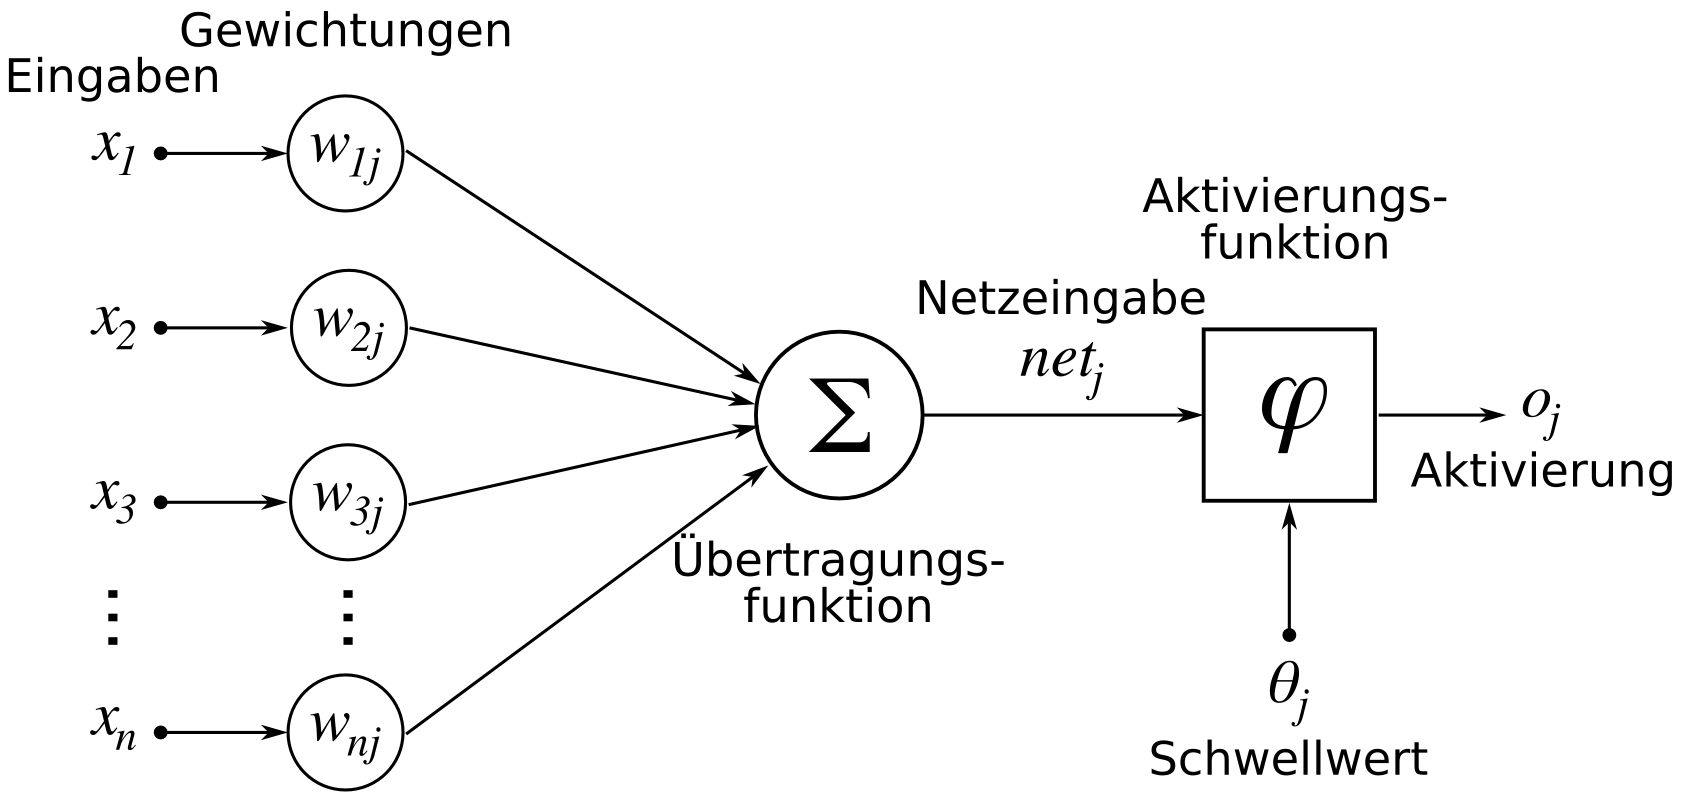
\includegraphics[width=0.8\textwidth]{Bilder/ArtificialNeuronModel_deutsch.png}\cite{das}\end{center}
Wie man auf der Abbildung erkennen kann wird in einem künstlichen Neuron die Summe der Produkte aus Gewichten und Eingaben durch die Aktivierungsfunktion zur nächsten Eingabe.
\subsubsection*{Aktivierungsfunktion}

	Aktivierungsfunktionen werden dazu benutzt um die Information einer Schicht des neuronalen Netzwerks zu verarbeiten um sie an die nächste Schicht weiterzugeben.\\

	Das Benutzen einer Aktivierungsfunktion ist von Vorteil, da so dem Neuronalen Netzwerk ermöglicht wird komplexere Probleme zu lösen. Ein Neuronales Netz ohne Aktivierungsfunktion zu trainieren ist trotzdem möglich, es könnte aber nur lineare Probleme lösen.
	%todo : Einfügen warum Modell nicht linear ist
	
	Deshalb werden im Maschinellen Lernen, wenn es mehrere Versteckte Schichten gibt oftmals Aktivierungsfunktionen benutzt.\\
	
\subsubsection*{Sigmoidfunktion} \label{Sig}
	Die Sigmoidfunktion ist die am häufigsten benutzte Aktivierungsfunktion, da sie eine nicht lineare Funktion ist. Sie kann folgendermaßen beschrieben werden:
	\begin{center}
	\large{f(x)= $\frac{1}{1+e^{-x}}$}
	
	\end{center}

Im Projekt wurde diese Sigmoidfunktion ebenfalls verwendet, da sie nicht linear ist, die Werte in einen Bereich zwischen 0 und 1 transformiert und ableitbar ist (vgl. \citeauthor{sharma2017activation} \citeyear{sharma2017activation} S.312 Abschnitt c )\\
\begin{center}


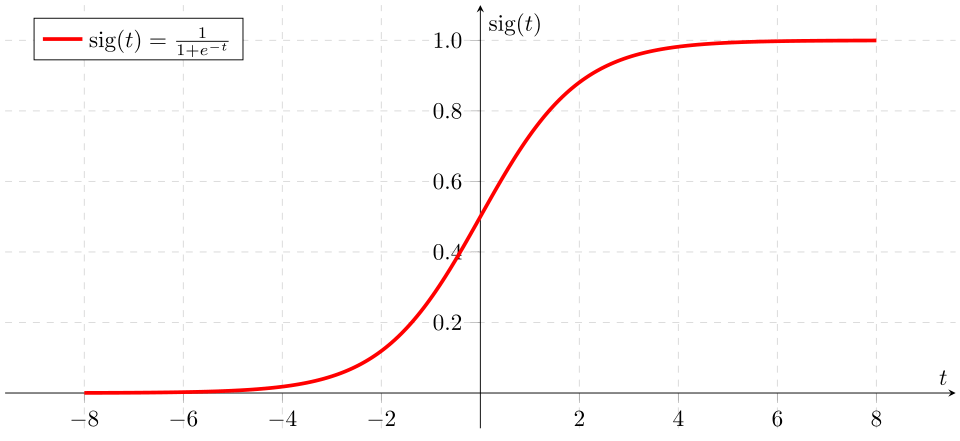
\includegraphics[width=0.8\textwidth]{Bilder/Sigmoid-function-2.png}\\
%todo
\textit{\small{Plot der Sigmoidfunktion im Intervall }[-8;8]}
\end{center}
Für zu große x-Werte kann es in Python zu einem \glqq Overflow Error" kommen. In diesem Fall wird f(x) zu Null wenn x kleiner 0 ist und zu Eins wenn x größer 0 ist. 
\section{Optimierungsfunktion}
Die Optimierungsfunktion ist im Projekt der Algorithmus, der die Gewichte des Neuronalen Netzes anpasst\footnote{Im Projekt die Methode: evaluieren(score)} nach der Form:\\
\begin{center}


\textit{Reward Increment = Nichtnegativer Faktor * Offset Reinforcement * Characteristic Eligibility} \cite[vgl.][S.234]{williams1992simple}\\ \textbf{oder}
\\
$\Delta w_{ij} = \alpha _{ij}(r-b_{ij})e_{ij}$\\
\end{center}
Wobei $\Delta w_{ij}$ die Gewichtsänderung darstellt, der nicht negative Faktor $\alpha _{ij}$ auch eine Konstante sein kann, die auch als Lernfaktor bekannt ist\footnote{Im Projekt: self.Lernfaktor = 3}, der 1.Summand \textit{r} die aktuelle Punktzahl, der 2.Summand \textit{b} die maximale Punktzahl aller Generationen und $e_{ij}$ ein Produkt
$e_{ij} =ln(f_{ij})\cdot{}\dfrac{1}{w_{ij}}$ mit $f_{ij}$, dem durch die Aktivierungsfunktion berechneten Ausgabe eines Neurons und $w_{ij}$ dem derzeitigen Gewicht des Neurons.\\
Diese Funktion hat jeden Durchgang eine Chance\footnote{ In der Methode maingameloop() mit der lokalen Variable \textit{ch} änderbar} aufgerufen zu werden, um das Neuronale Netz zu aktualisieren.\label{OptF}
\subsubsection*{Probleme der Optimierungsfunktion}
Wenn \textit{b} gleich \textit{r} wird die ganze Gleichung 0, somit kann kein weiteres Lernen mehr stattfinden.

\section{Probleme des Bestärkenden Lernens}
Beobachtet man den maximalen Score des Spielers in der derzeitigen Konfiguration über mehrere Generationen und Anläufe hinweg so stellt man fest, dass dieser selten, wenn nicht sogar nie, über 5 Punkte hinausgeht. Jetzt muss man nach den Problemen suchen, die verhindern, dass der Agent mehr lernt.
\subsection{Underfitting}
Underfitting (deutsch Unteranpassung) ist ein Problem, das im bestärkenden Lernen auftreten kann, wenn das Modell weniger komplex ist, als die Daten mit denen es zu arbeiten versucht\cite[vgl.][S.6-7]{koehrsen2018overfitting}. Dies ist zu Beispiel der Fall, wenn man versucht ein lineares  Modell auf ein nicht lineares Problem anzuwenden. Dies ist bei dem hier verwendeten Neuronalen Netzwerk nicht der Fall, da die in \ref{Sig} beschriebene Aktivierungsfunktion nicht linear ist und somit das Modell komplex genug sein sollte, um Space Invaders zu schlagen.

\subsection{Overfitting}
Was eher der Fall sein könnte ist eine Art des sogenannten Overfittings, das im Deutschen als Überanpassung bekannt ist. Hierbei passt der Agent seine Strategie zu genau an das Problem an und probiert keine neuen Strategien mehr aus. Dieser Fall tritt hier ein, wenn der Spieler lernt nur zu schießen, weil er damit eine Punktzahl von 5 erreicht und diese höher ist als die vorherige Punktzahl. Eine Möglichkeit dieser Überanpassung vorzubeugen besteht darin, dass Problem leicht zu variieren. Zum Beispiel kann man die Monster jede Runde zufällig platzieren.\footnote{ Dies passiert wenn man in der reset-Funktion die lokale Variable  random auf False setzt}. Dies kann aber auch zu Folge haben, dass der Agent das Problem zufällig löst. Auch könnte dieses Problem gelöst werden, indem man die Belohnung an die vergangene Zeit koppelt, ähnlich wie ich noch in \ref{D1} erklären werde.